%%%%%%%%%%%%%%%%%%%%%%%%%%%%%%%%%%%%%%%%%%%%%%%%%%%%%%%%%%
%                                                                                      %
%         Bristol Project LaTex Template            %
%                                                                                      %
%%%%%%%%%%%%%%%%%%%%%%%%%%%%%%%%%%%%%%%%%%%%%%%%%%%%%%%%%%
%
%   Author: Alex Charles           Email: aep.charles@gmail.com
%
% -----------------------------------------------------------------------------------
%      PACKAGES & OTHER DOCUMENT CONFIGURATIONS
% -----------------------------------------------------------------------------------
\documentclass[10pt]{article}
\usepackage[utf8]{inputenc}
\usepackage[T1]{fontenc}
\usepackage[british]{babel}
% ----------NEW BIBLATEX BIBLIOGRAPHY-----------------------------------------------
\usepackage[backend=bibtex,style = ieee]{biblatex} % Upgrades Bibliography

\addbibresource{BibFile.bib} %%% For biblatex
%e.g to add page number \footfullcite[chapter, p.~215]{AAIB}
% This allows can use footfullcite commands
% Note urldate field must be in yyyy-mm-dd to work - use online type
% Remeber to use \printbibliography in the footer
% -----------------------------------------------------------------------------------
\usepackage{sectsty}
\usepackage{amssymb,amsmath}
\usepackage{ifxetex,ifluatex}  %<<<<<<<<< Edit FONT HERE
\ifnum 0\ifxetex 1\fi\ifluatex 1\fi=0 % if pdftex
  \usepackage[T1]{fontenc}
  \usepackage[utf8]{inputenc}
\else % if luatex or xelatex
  \ifxetex
    \usepackage{mathspec}
    \setmainfont{Avenir-Light}
  \else
  % Font Package for XeLatex
    \usepackage{fontspec}
    \setmainfont{Avenir-Light}
  \fi
  \defaultfontfeatures{Ligatures=TeX,Scale=MatchLowercase}
\fi
\usepackage[fit]{truncate} %Truncates headers that are too long
\usepackage{fancyhdr}
\usepackage{lastpage}
\usepackage{extramarks}
\usepackage{gensymb}
\usepackage{lipsum}
\usepackage{float}
\usepackage{graphicx}
\graphicspath{{TempImg/}{Img/}}%<<<<<<<<< Location of Template Images and Other Images, Add folders here
\usepackage{subfig}
\usepackage{wrapfig}
\usepackage[font ={small,it}]{caption}
\usepackage{refcheck} %Check references
\usepackage{amsfonts,amsthm} % Math packages
% \usepackage{cite}
% \usepackage[maxlevel=3]{csquotes}
%    \MakeAutoQuote{‘}{’}
%    \MakeAutoQuote*{“}{”} %corrects quote marks
\usepackage{enumitem} % resume numbered lists
\usepackage{multicol} %for mulitple colums in lists
\usepackage{geometry}
\usepackage{booktabs} %<<<<<<<<< Table drawing package
\usepackage[table,xcdraw]{xcolor} %<<<<<<<<< Table drawing package
\usepackage{svg}
\usepackage{scrextend} %call footnotes
\usepackage[colorlinks, linkcolor = black, citecolor = black, filecolor = black, urlcolor = blue]{hyperref} % Creates Hyperlinks for references - add [colorlinks] for coloured hyperlinks
\usepackage{changepage} %Allows Adjust width to be used for the document (indenting paragraphs)
\usepackage{pdfpages} %Allows Pdfpages to be added to the document use \includepdf[pages={1}]{myfile.pdf}
\usepackage{pdflscape} %Change Pages from Portrait to Landscape

\usepackage[compact]{titlesec}
% \titlespacing*{\section}{0pt}{1.1\baselineskip}{\baselineskip}

\renewcommand*{\thefootnote}{\alph{footnote}} %%% Changes footnotes to letters
\usepackage[bottom]{footmisc} %%% Pushes footnote to bottom and to the margin

\DeclareCiteCommand{\footcite}[\mkbibfootnote]
{\usebibmacro{cite:init}%
\usebibmacro{prenote}}
{\usebibmacro{citeindex}%
\printtext[brackets]{\usebibmacro{cite:comp}}}
{\multicitedelim}
{\usebibmacro{cite:dump}%
\usebibmacro{postnote}}

\newenvironment{indentpara}{\begin{adjustwidth}{2cm}{}}{\end{adjustwidth}} %Declare adjust width wiht indentpara
\renewcommand{\labelitemii}{$\circ$}
\renewcommand{\labelitemiii}{$\diamond$}
\renewcommand{\labelitemiii}{$\cdot$}

% -----------------------------------------------------------------------------------
%                 Quotes
% -----------------------------------------------------------------------------------

\usepackage{epigraph}
% \epigraphsize{\small}% Default
\setlength\epigraphwidth{12cm}
\setlength\epigraphrule{0pt}

\usepackage{etoolbox}
\apptocmd{\sloppy}{\hbadness 10000\relax}{}{}%%%% > Removes Url bibliography warnings
\makeatletter
\patchcmd{\epigraph}{\@epitext{#1}}{\itshape\@epitext{#1}}{}{}
\makeatother

%%%% > For Quotes Use \epigraph{"Quote"}{ - \textup{Author}, Book}

% -----------------------------------------------------------------------------------
%                   NAMES & CLASS DEFINITION %<<<<<<<<< INSERT DETAILS HERE
% -----------------------------------------------------------------------------------
\newcommand{\AssignmentTitle}{Investigation of the Use Energy Storage Technologies to Reduce Peak Demand Charges for the University of Bristol}
\newcommand{\ModuleTitle}{Design Project 4 - Interim Report}
\newcommand{\University}{University of Bristol}
\newcommand{\Faculty}{Faculty of Engineering}
\newcommand{\UniCrest}{crestbris.png}
\newcommand{\UniLogo}{logobris.png}%<<<<<<<<< Make Sure Files are in the Template
%\newcommand{\GroupName}{Group 2}
\newcommand{\StudentNameA}{Alex Charles}
\newcommand{\StudentNumberA}{67634}
\newcommand{\SupervisorNameA}{Dr Theo Tryfonas}
\newcommand{\SupervisorEmailA}{Theo.Tryfonas@bristol.ac.uk}
% \newcommand{\SupervisorNameB}{Name}
% \newcommand{\SupervisorEmailB}{email@gmail.com}

% -----------------------------------------------------------------------------------
%        PACKAGES FOR MARKDOWN CONVERSION - FOR USE If Using Markdown to Latex
% -----------------------------------------------------------------------------------
\usepackage{fixltx2e} % provides \textsubscript
% use upquote if available, for straight quotes in verbatim environments
\IfFileExists{upquote.sty}{\usepackage{upquote}}{}
% use microtype if available
\IfFileExists{microtype.sty}{%
\usepackage{microtype}
\UseMicrotypeSet[protrusion]{basicmath} % disable protrusion for tt fonts
}{}
\hypersetup{unicode=true,
            pdftitle={\AssignmentTitle},
            pdfauthor={\StudentNameA},
            pdfborder={0 0 0},
            breaklinks=true}
\urlstyle{same}  % don't use monospace font for urls
\usepackage{fancyvrb}
\VerbatimFootnotes % allows verbatim text in footnotes
\usepackage{longtable,booktabs}
\IfFileExists{parskip.sty}{%
\usepackage{parskip}
}{% else
\setlength{\parindent}{0pt}s
\setlength{\parskip}{6pt plus 2pt minus 1pt}
}
\setlength{\emergencystretch}{3em}  % prevent overfull lines
\providecommand{\tightlist}{%
  \setlength{\itemsep}{0pt}\setlength{\parskip}{0pt}}
% \setcounter{secnumdepth}{0}
% Redefines (sub)paragraphs to behave more like sections
\ifx\paragraph\undefined\else
\let\oldparagraph\paragraph
\renewcommand{\paragraph}[1]{\oldparagraph{#1}\mbox{}}
\fi
\ifx\subparagraph\undefined\else
\let\oldsubparagraph\subparagraph
\renewcommand{\subparagraph}[1]{\oldsubparagraph{#1}\mbox{}}
\fi

% -----------------------------------------------------------------------------------
%                   WORD COUTNER - for XeLaTex
% -----------------------------------------------------------------------------------
\usepackage{xesearch}
\newcounter{words}
\newenvironment{counted}{%
  \setcounter{words}{0}
  \SearchList!{wordcount}{\stepcounter{words}}
    {a?,b?,c?,d?,e?,f?,g?,h?,i?,j?,k?,l?,m?,
    n?,o?,p?,q?,r?,s?,t?,u?,v?,w?,x?,y?,z?}
  \UndoBoundary{'}
  \SearchOrder{p;}}{%
  \StopSearching}

% -----------------------------------------------------------------------------------
%                   MARGINS, HEADERS & FOOTERS
% -----------------------------------------------------------------------------------
 \geometry{
 left=20mm,
 right=20mm,
 top=25mm,
 bottom=25mm,
 }
\linespread{1.4}

\pagestyle{fancy}
\lhead{\includegraphics[width = 0.2\textwidth]{\UniLogo}}
% \chead{\AssignmentTitle}
% \rhead{}
\lfoot{\StudentNameA}
\cfoot{}
\rfoot{Page \thepage} %%%% note the footer is swapped when page numbering style changes
\renewcommand\headrulewidth{0.4pt}
\renewcommand\footrulewidth{0.4pt}

\setlength\parindent{0pt}

\newcommand{\horrule}[1]{\rule{\linewidth}{#1}}

% -----------------------------------------------------------------------------------
%               DOCUMENT STRUCTURE COMMANDS
% -----------------------------------------------------------------------------------
% To sort out the formatting of header and footer when a page...
% ... split occurs "within" a problem environment.
\newcommand{\enterProblemHeader}[1]{
\nobreak\extramarks{#1 (Cont.)}\nobreak
\nobreak\extramarks{#1}{}\nobreak
}
% To sort out the formatting of header and footer when a page...
% ... split occur "between" problem environments.
\newcommand{\exitProblemHeader}[1]{
\nobreak\extramarks{#1 (Cont.)}\nobreak
\nobreak\extramarks{#1}{}\nobreak
}

% -----------------------------------------------------------------------------------
\begin{document}

  \setlength{\abovedisplayskip}{-18pt}
  \setlength{\belowdisplayskip}{0pt}
  \setlength{\abovedisplayshortskip}{-18pt}
  \setlength{\belowdisplayshortskip}{0pt}

  \setlist[enumerate]{itemsep=-2mm}


%----------------------------------------------------------------------------------------
                                  %	TITLE PAGE FORMAT
%----------------------------------------------------------------------------------------
\pagenumbering{roman}
\begin{titlepage}

	\center % Center everything on the page
%----------------------------------------------------------------------------------------
%	HEADING SECTION
%----------------------------------------------------------------------------------------
		\usefont{OT1}{bch}{b}{n}
		\normalfont \normalsize \textsc{\University} \\ [10pt]
		\normalfont \normalsize \textsc{\Faculty} \\ [25pt]
%----------------------------------------------------------------------------------------
%	LOGO SECTION - Adds Univeristy Crest to the Report
%----------------------------------------------------------------------------------------
\newcolumntype{C}{>{\centering\arraybackslash} m{6cm} }  %# New column type
\begin{tabular}{CC}
  \includegraphics[width = 0.2\textwidth]{\UniCrest} &   \includegraphics[width=0.3\textwidth]{Arup_logo.png}
\end{tabular}\\[0.5cm]
%----------------------------------------------------------------------------------------
%	HEADING SECTION
%----------------------------------------------------------------------------------------
		\normalfont \normalsize \textsc{\ModuleTitle} \\ [25pt]
%----------------------------------------------------------------------------------------
%	TITLE SECTION
%----------------------------------------------------------------------------------------
		\horrule{0.5pt} \\[0.4cm]
		\huge \textbf{\AssignmentTitle} \\
		\horrule{2pt} \\[0.5cm]
%----------------------------------------------------------------------------------------
%	HEADING SECTION
%----------------------------------------------------------------------------------------
%		\normalfont \normalsize \textsc{\GroupName} \\ [25pt]
%----------------------------------------------------------------------------------------
%	AUTHOR SECTION
%----------------------------------------------------------------------------------------
\begin{minipage}{0.4\textwidth}
\begin{flushleft} \large
\emph{Supervisors:}\\
% Change Name
\textbf{\SupervisorNameA}\\
% \textbf{\SupervisorNameB}
\end{flushleft}
\end{minipage}
~
\begin{minipage}{0.4\textwidth}
\begin{flushright} \large
\emph{Email:} \\
\SupervisorEmailA\\
% \SupervisorEmailB

\end{flushright}
\end{minipage}\\[1cm]

\begin{minipage}{0.4\textwidth}
\begin{flushleft} \large
\emph{Author:}\\
	\textbf{\StudentNameA}
\end{flushleft}
\end{minipage}
~
\begin{minipage}{0.4\textwidth}
\begin{flushright} \large
\emph{Candidate Number:} \\
(\StudentNumberA)\\
\end{flushright}
\end{minipage}\\[2cm]

%----------------------------------------------------------------------------------------
%	DATE SECTION
%----------------------------------------------------------------------------------------
\textit{{\large \today}}\\[1cm] % Date, change the \today to a set date if you want to be precise
%----------------------------------------------------------------------------------------
\vfill % Fill the rest of the page with whitespace
\end{titlepage}

% \setcounter{page}{3}

\newpage


% -----------------------------------------------------------------------------------
%                             	 ABSTRACT
% -----------------------------------------------------------------------------------

% -----------------------------------------------------------------------------------
%                              TABLE OF CONTENTS
% -----------------------------------------------------------------------------------

\tableofcontents


% \newpage
% \addcontentsline{toc}{section}{List of Acronyms}
% \section*{List of Acronyms}\label{acronyms}
% \textbf{BRB}: Be Right Back \\


% \newpage

% \addcontentsline{toc}{section}{Acknowledgements}
% \section*{Acknowledgements}\label{acknowledgements}

% \addcontentsline{toc}{section}{Declaration}
% \section*{Declaration}\label{declartion}
% I hereby declare that this report entitled “\AssignmentTitle” submitted to Bristol University, is a record of an original work completed by myself.\\

% \newpage

%% -----------------------------------------------------------------------------------
%%                          	  INTRODUCTION
%% -----------------------------------------------------------------------------------
\clearpage
\rfoot{Page \thepage\ of \pageref{LastPage}}
\pagenumbering{arabic}
\begin{counted} %<<<<<<<<<<<<<<STARTS WORD COUNTER
\section{Aims and Objectives}\label{aims-and-objectives}

The announcement of the new £300million University of Bristol Campus in
Temple Quarter \cite{November58:online}, presents an exciting new
opportunity for development of digital innovations in sustainable
energy. The government's 2020 smart meter rollout, is the first step for
creating a smart energy grid, key to achieving a low-carbon, efficient
energy for the UK \cite{SmartEne79:online}. The UK's vision is inline
with the University of Bristol's new strategy, seeking to boost it's
world-class research capacity and promote policy innovation in
sustainability \cite{universi93:online}. Create a world leading
sustainable digital campus, holds as an attractive means for the
University to achieve it's vision. Consequently, aim of the group
project is to bring a host of new digital technologies reducing both
energy costs and energy usage, uniting these themes, to radically
increase the new campus's sustainability.

\begin{figure}[H]
\centering
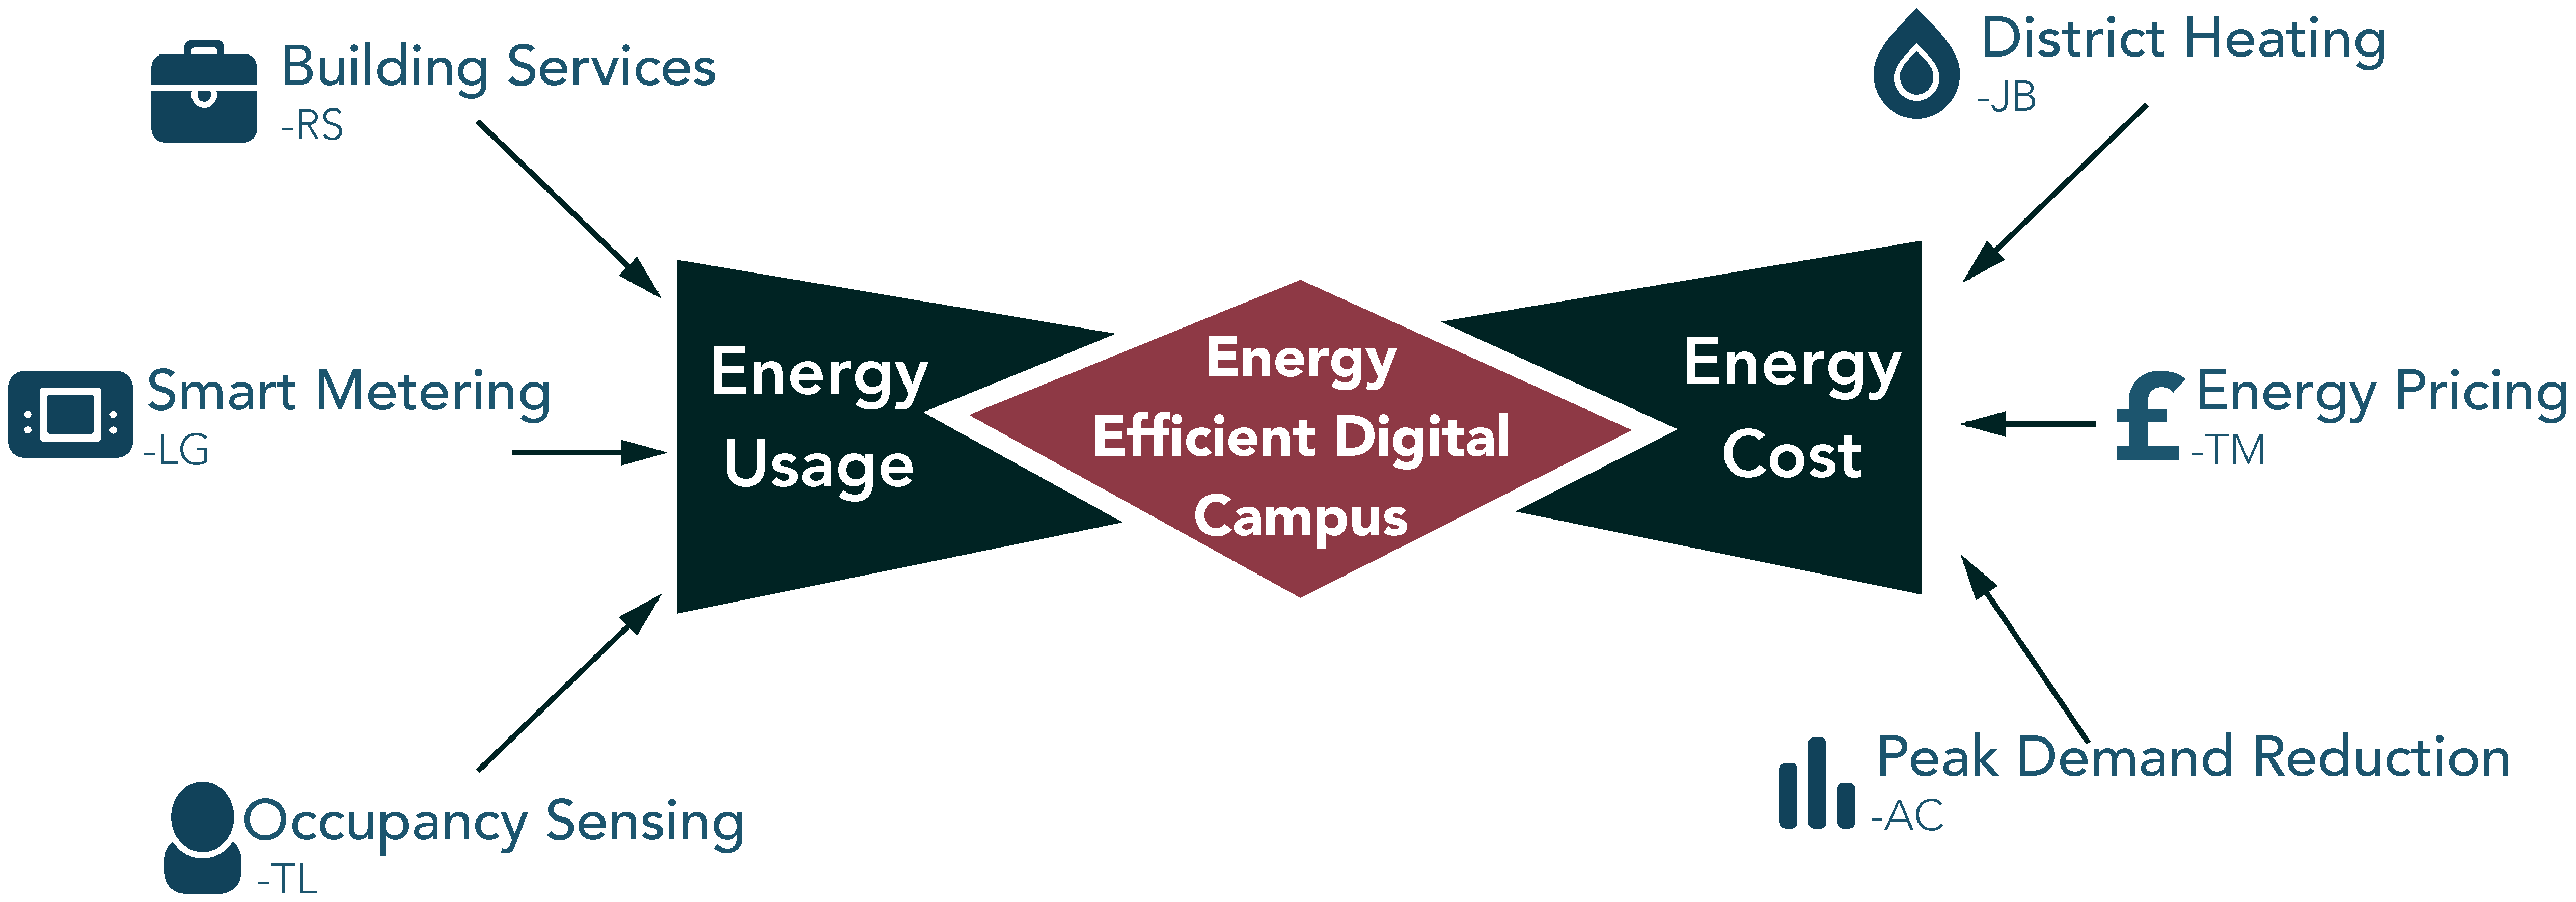
\includegraphics[width=1\textwidth]{groupDia}
\caption{Group Design Project Diagram Showing Relationships Between Individual Projects}
\label{groupDia}
\end{figure}

Figure \ref{groupDia} shows how the separate themes of the project are
split, where research in Occupancy Sensing, Smart Metering and Building
Services will evaluate how energy usage in the new campus can be
optimised. District Heating, Energy Pricing and Peak Demand Reduction,
all analyse methods of reducing energy costs for the University. Where
new energy pricing structures coupled with peak demand reduction
technologies, can reduce the load on the grid, helping support
sustainable energies. When these separate streams are brought together
in 5\textsuperscript{th}\^{} year, a smart ``brain'' will be created,
combining usage data with reduction in energy costs to provide
sustainable energy services to the campus in that will push the
University to meet it's carbon neutral 2030 goal
\cite{universi93:online}.

\subsection{Individual Project Aim}\label{individual-project-aim}

The aim of this individual project is to investigate the feasibility of
a battery energy storage system to reduce peak energy demand charges for
a new University of Bristol campus. The University's peak demand charges
will be analysed and simulated, showing how peak demand is charged in a
normal use case. Different peak shaving system architectures will then
be added to the model, to find an optimum solution for the system's
design with respect to the system capital cost against peak demand
charge savings. A comparison between using a micro system, for room by
room use, or a macro system, being applied to the whole campus will be
conducted. The outputs of the project for 5\textsuperscript{th} year
will be a flexible model which produces an optimum peak shaving system
architecture for a given University scenario.

\subsection{Objectives}\label{objectives}

\textbf{Literature Review}

\begin{enumerate}
\item Research different peak shaving systems available on the market and similar systems designs in literature, highlighting relevant modelling techniques and limitations.
\item Perform a detailed literature review to investigate applicable peak shaving technologies based on similar use cases and performance. Research will include:
    \begin{itemize}
 \item a down-selection of different energy storage solutions, looking at their applicability to a University peak shaving system, comparing parameters such as; power-ratings , discharge times, charge times and costs.
\item investigating different prediction methods for peak demand surges, identifying limitations in current technology.
    \end{itemize}
\end{enumerate}

\textbf{Definition of System Architectures}

\begin{enumerate}[resume]
\item Define peak shaving system architectures, establishing the key performance variables.
\end{enumerate}

\textbf{Modelling and Analysis}

\begin{enumerate}[resume]
\item Analyse the University’s current peak demand charges. This will include understanding the University’s current demand charge structure and collecting typical energy usage data. Parameters such as time of day and sources of energy peaks will be included.
\item Produce a simulation to optimise the peak shaving system, comparing metrics including; unit cost and reduction in peak kWh charges based on University billing structure. This model will provide a comparative analysis between the different system architectures. This will detail savings against the University’s current peak demand charges. The model will be comprised of three stages:
\begin{enumerate}
\item A simulation of the University's a normal energy use case and peak demand charges, for use as a datum.
\item Inclusion of energy storage systems, simulating logic and detailing any prediction methods.
\item Addition of other factors to improve the model, taken from the literature review. This will take into other technologies such as peak load shedding to understand if peak demand can be further reduced.
\end{enumerate}
\item Analyse others areas where the system could deliver further benefits, such as AC to DC conversion, PV’s, micro-grids and increased sustainability.
\end{enumerate}

\textbf{Evaluation}

\begin{enumerate}[resume]
\item Evaluate results of the simulation, concluding on the effectiveness of different peak shaving system architectures against particular scenarios.
\end{enumerate}

\newpage

\section{Background and Summary of Key Work and
References}\label{background-and-summary-of-key-work-and-references}

The following literature review provides a comprehensive overview of
current research into using Energy Storage Systems (ESS) to reduce peaks
in energy demand and lower utility costs for the consumer. Peak demand
reduction is synonymous with peak shaving; the ability to control energy
usage from a supplier during intervals of high demand, to limit or
reduce demand charges\cite{schneiderRECPS}. As this project is
investigating reducing the peak demand charge for the University of
Bristol, a thorough understanding of the charging structure is given in
section \ref{peak-demand-charges}, providing context for the system to
solve. Section
\ref{current-peak-demand-management-methods-and-energy-storage-systems-usage}
evaluates traditional methods of peak shaving, covering a brief look at
ESS's current usage. Section
\ref{peak-shaving-systems-literature-review} includes a broad range of
research around using ESS in different case studies, optimising the
system architecture and analysis on ESS's financial return on investment
(ROI). This research will help in defining the system architecture to be
modelled, highlighting relevant modelling techniques to consider while
showing the limitations in current research. Finally section
\ref{peak-shaving-technologies---electrical-storage-system-ess} analyses
the applicability of different ESS's, down-selecting to leave a
shortlist of ESS's to be modelled.

\subsection{Peak Demand Charges}\label{peak-demand-charges}

The University of Bristol's infrastructure, spans across three sites;
the City Centre, Stoke Bishop and Langford. Across these places, the
majority of facilities receive separate energy bills, allowing a high
degree of granularity in the understanding energy charges
\cite{Jbrentmeet}. These costs are broken down into several factors,
where many separate bills are bundled together under the same theme
\cite{Jbrentmeet}. These different charges are:

\begin{multicols}{2}
\begin{enumerate}
\item Unit Charge
\item Distribution Use of System (DUoS)
\item Feed-In Tariff (FIT)
\item Transmission Network Use of System (TNUoS)
\end{enumerate}
\end{multicols}

The charges that peak-shaving system will target are DUoS, TNUoS and
Unit Cost (by secondary means). DUoS charges include the capacity
charge; where the customer pays for a maximum energy demand level that
the institution will not exceed \cite{Deconstr52:online}. The capacity
charge is set at a bar higher than the actual maximum demand, reducing
the risk of breaching this threshold. If breached, the customer incurs
substantial penalties, and the supplier increases the threshold for the
next billing period. By levelling off peaks in energy demand, the
capacity charge threshold can decrease; this will be the key focus for
the peak-shaving system.

TNUoS charges come from three half-hour periods when the UK's National
Grid energy demand is greatest, referred to as Triads. These dates lie
between November and February and must be separated by at least ten days
during the financial year, calculated yearly \cite{TriadsWh7:online}.
The average maximum (peak) demand across the three Triad periods
\cite{TNUoSTra99:online}, is multiplied by tariff in the respective zone
in cost per kW \cite{TNUoScha93:online}. Combined they become the TNUoS
charge, added to the customer's end of year bill. Being able to
radically reduce peaks through using ESS or generation in these periods
will reduce the bills cost significantly.

Energy unit costs come at three different rates, green, amber and red
\footcite[See page 27 of][]{SWEB201492:online}, depending on the time of
day; where energy usage in red periods are significantly higher
(generally between 5pm-7pm). Section \ref{forecasting} discusses
literature around these charges.

\subsection{Current Peak Demand Management Methods and Energy Storage
Systems
Usage}\label{current-peak-demand-management-methods-and-energy-storage-systems-usage}

Traditionally there are two methods for reducing peak demand for
industrial complexes. These are:

\begin{itemize}
\tightlist
\item
  \textbf{Load Shedding}: This is reducing energy usage, by
  understanding which parts of the system can be switched off during
  periods of peak demand \cite{6199851}. Scheduling can be an
  intelligent system or use simple forecasting tool
  \cite{Reducing37:online}. Often load shedding is calculated daily
  using a schedule to set the maximum limit; assuming that this limit
  will not change during the day \cite{6938948}.

  \begin{itemize}
  \tightlist
  \item
    \emph{Limitations}: This method can typically lead to significant
    forecasting errors were reactive methods are often is better
    \cite{6938948}. Due to the free flow of staff and students at the
    University's facilities, predicting peak demands accurately can
    become a greater challenge.
  \end{itemize}
\item
  \textbf{On-site Generation}: Adding of the grid capacity to the
  consumer \cite{schneiderRECPS}. The university currently uses some
  generators to reduce red zone unit charges.

  \begin{itemize}
  \tightlist
  \item
    \emph{Limitations}: The University currently has 0.5MW of
    PhotoVoltaic (PV) installed using nearly all available space. These
    PV's make up only 0.5\% of the total energy demand \cite{Jbrentmeet}
    meaning on-site generation to offset peak demand has a negligible
    effect in flattening the University's demand in it's standard form.
  \end{itemize}
\end{itemize}

Due to these limitations and statistics such as ``40\% of energy use in
the campus comes from 5\% of the space, predominantly labs''
\cite{brentemail}, make the University an interesting case study how
developments in ESS, could present a better method of reducing peak
demand charges.

There are a limited number of peak shaving ESS solutions available
commercially. ABB offers energy-storage, smart-grid products, perform
load levelling at grid level \cite{abbpeakshave}. These systems are
designed primarily for supply levelling, using forecasting methods and
large electrical storage systems to offset excess energy supply produced
from renewable energies \cite{5559470}, rather than targeting bill
reduction for its' customer. One Cycle Control have created technologies
to regulate peak-load and mitigate peak demand charges for
commercial/industrial facilities using Li-ion batteries
\cite{peakload38:online}. The technologies proved effective at reducing
peak demand charges, but the cost of the ESS \cite{Demonstr51:online}
reduces their financial feasibility. It is clear that the ESS selected
the most important factor regarding the systems cost while being able to
sense peak loads and respond actively will maximise the performance of
the system. Section
\ref{peak-shaving-technologies---electrical-storage-system-ess}
evaluates these two different technologies.

\subsection{Peak Shaving Systems Literature
Review}\label{peak-shaving-systems-literature-review}

Acknowledging limitations in commercial ESS technology, a literature
review was performed investigating research relevant to designing a
peak-shaving system architecture using an ESS. Research is grouped,
highlighting each section's significance to achieving the objectives of
the project.

\subsubsection{Forecasting and ESS in Load
Shifting}\label{forecasting-and-ess-in-load-shifting}

By understanding when energy prices will be greater and when loads are
typically larger, an ESS can be switched on during these periods to
reduce demand from the grid. Energy costs are shifted, purchasing energy
at cheaper rates and using this energy during peak times. For western
power, there is a 17000\% increase in price during this period
\footcite[25.405 p/kWh in red times to 0.147p/kWh in green times][]{SWEB201492:online}.
Looking at the gap in energy prices, demand charges and investment costs
for an ESS, for NaS, Li-ion and Flow batteries, a basic on/off algorithm
to shift energy purchasing from peak to off-peak times does not produce
a viable return on investment (ROI) \cite{7555795}. \cite{7555793}
highlights that billing peak periods were directly correlated with peak
demand, requiring large ESS to offset this demand. \cite{5590194} used
real hourly spot prices to decide the best times to turn on and off
Vanadium Redox Batteries (VRB) and Polysulfide Bromide Batteries (PSB).
Through sequential quadratic programming (SQP), battery sizes were
optimised, finding PSB's had a better business case for load shifting.
The fundamental differences between \cite{5590194} and \cite{7555795},
were the reduction in the size of the problem and the granularity of the
pricing data used. \cite{shen2016} and \cite{6461115} both look at
different modelling techniques to simulate load shifting with EES. Using
an agent-based simulation, \cite{6461115} was able to reduce the
diversity in load consumptions patterns, consequently reducing peak
demand, creating an active market to trade energy demand.
\cite{shen2016} looked at how the peak rebate scheme may lower ROI for
ESS's. Neither modelling methods are appropriate for this project.
\cite{6938948} evaluated different control strategies combining many
forecasts to reduce errors in peak shaving over a monthly period.
Weighted and lowest error forecasts were the best strategies for an
energy management system and should be added to the system architecture
if forecasting is used. \cite{Bennett2015122} added a real-time operator
to create and intelligent scheduling system based on a house to
forecast. This system significantly improved the state of charge of the
battery, allowing more energy available to reduce peaks, highlighting
that forecasts combined with real-time information can increase the
performance of the system further.

\subsubsection{Supply Levelling}\label{supply-levelling}

Supply levelling has been the most common use for ESS
\cite{iearoadmapes}, using large batteries to reduce power fluctuations
brought by the use of renewable technologies. Supply levelling works by
storing excess supply, reducing peaks in supply rather than in demand.
The technology is, therefore, similar to peak shaving.
\cite{Allik20161116} looked at improving supply on the micro (house)
scale. Shiftable water heating was used as the primary storage device in
houses, accounting for 50\% of household electricity use. Excess load
from wind turbines can be used to heat water in these periods bypassing
an inverter making a more efficient use of the external energy.
Minimising conversion through invertors makes a large difference in the
efficiency of the system.

\subsubsection{Battery Sizing and Financial
Modelling}\label{battery-sizing-and-financial-modelling}

There have been numerous studies conducted looking into the business
cases for ESS's. \cite{7555795} and \cite{7555793} model a broad use of
using ESS's to reduce the cost of all energy charges, finding that the
ROI is unlikely to be feasible until 2020. Papers including
\cite{1300158} and \cite{6175723} evaluated financial models for
particular case studies, showing that bespoke solutions achieved greater
peak shaving reductions than returns promised by current generic
products \cite{abbpeakshave}. \cite{7555795}, \cite{7555793},
\cite{1300158} and \cite{6175723} enable a strong argument that a
bespoke solution for the University offer a better business case for ESS
than commercial technology.

Investigating the benefits of a decentralised system, reducing peaks on
a small scale rather than using one large central ESS, \cite{6604477}
analysed both peak shaving and battery longevity for a large data
centre. The ability to forecast when a machine will spike in power usage
follows a similar to people within a building. Through both
experimentation and modelling, \cite{6604477} showed that when regarding
the batteries lifespan, the ability to regulate load through a series of
batteries can be more favourable than a centralised system.
\cite{Demonstr51:online} supports using a decentralised system. A
simulation of the impact of lithium-ion batteries operated under a
peak-shaving control algorithm identified the cost-optimal battery
configurations, and their impact on grid demand revealing that small
short duration batteries was more favourable and cost effective for the
customer. The model for this project will assess if this is also the
case for a University facility understanding that a few rooms such as
labs contribute to the majority of peak loads.

\cite{20160601898032}, \cite{Levron201280} all \cite{5371839} all show
alternate ways of optimising the battery sizing configurations.
\cite{5371839}, used a non-numeric modelling method, focusing on
ultra-capacitors to find the optimal ESS. The results emphasised the
constraint of storage capacity, showing that limited value is gained
after a particular size of ESS is used. Finding this size for the
University will be the primary focus of this projects model.
\cite{Levron201280} created an analytical modelling, leveraging
intuitive energy bands to regulate the peak load giving an optimum
storage size for a given system, a simple and effective method of
modelling battery usage. \cite{20160601898032} looked specifically at
Vanadium Redox Flow Batteries (VRFB) arguing it benefits over other ESS
methods. A MATLAB/Simulink was made for a residential use case, showing
that VRFB can regulate it's frequency efficiently, due to its fast
response time, while still performing peak-shaving services. A more
specified approach to \cite{20160601898032} model is proposed for this
project.

\subsection{Peak Shaving Technologies - Electrical Storage System
(ESS)}\label{peak-shaving-technologies---electrical-storage-system-ess}

The chosen Electrical Storage System (ESS) is the chief technology which
will affect the cost and feasibility of a peak shaving system, where of
these technologies are not suitable for a University peak-shaving
system. An ESS converts electrical energy into a form stored for later
use \cite{Chen2009291}. Electrochemical batteries characterise a
pollution-free operation, low maintenance, high round-trip efficiency,
long cycle lives, batteries arguably being the most appropriate
technology for peak shaivng\cite{liao2016a} \cite{Dunn928}. These have
been chosen as the main focus for this study. The various storage
methods can be characterised for different uses summaries below:

\begin{itemize}
\tightlist
\item
  \textbf{Energy Management:} for large scale storage, these are
  typically used by power plants for load levelling, ramping/load
  following, and spinning reserve.

  \begin{itemize}
  \tightlist
  \item
    Pumped Hydroelectric Storage (PHS), Compressed Air Energy Storage
    (CAES) and Cryogenic Energy Storage (CES) are the conventional
    technologies for high generation above 100MW. All these methods are
    on a scale too large to be considered for this project.
  \item
    Large-scale batteries, flow batteries, fuel cells, solar fuels, CES
    and Thermal Energy Storage (TES) are suitable for medium-scale
    energy management with capacities of 10--100 MW. These are
    appropriate for consideration for this project.
  \end{itemize}
\item
  \textbf{Power quality:} For fast response times for power quality such
  as the instantaneous voltage drop, flicker mitigation and short
  duration uninterrupted power supply

  \begin{itemize}
  \tightlist
  \item
    Flywheels, Batteries, Superconducting Magnetic Energy Storages
    (SMES), capacitors and supercapacitors have millisecond response
    time lower for storage sizes less than 1 MW - suitable perhaps in
    addition to large scale battery, flywheel efficiency, however, is
    too low for operational use, so has been removed from this study.
  \end{itemize}
\item
  \textbf{Bridging power:} Relatively fast response (\textless{} 1 s)
  but also have relatively long discharge time (hours). The typical
  power rating for these types of applications is about 100 kW--10 MW.

  \begin{itemize}
  \tightlist
  \item
    Batteries, flow batteries, fuel cells and Metal-Air cells
    \cite{Chen2009291}
  \end{itemize}
\end{itemize}

By removing energy storage methods that would not be appropriate for the
system, a table was created to compare the differing technologies,
included in the appendix. Batteries along with capacitors provide the
response time and efficiencies required to make the system justifiable,
where only rechargeable batteries were compared. From section
\ref{battery-sizing-and-financial-modelling} a model of a University
peak demand reduction system will need to compare different battery
parameters along with their cost, to optimise the model.

\newpage

\section{Project Work-plan}\label{project-work-plan}

This section describes the breakdown of the different work packages
required to complete the aims and objectives set out in section
\ref{aims-and-objectives}.

\paragraph{Work Package 1: Literature Review (Objectives 1 and
2)}\label{work-package-1-literature-review-objectives-1-and-2}

\begin{enumerate}[ label={1.\arabic*}]
\item Understand the University's energy pricing structure, defining the problem the peak shaving system will solve.
\item Perform a market survey of peak shaving systems available commercially and review literature of relevant research around peak shaving systems.
\item Evaluate different energy storage systems, looking at metrics including; power-ratings , discharge times, charge times and costs. Producing a shortlist of relevant ESS's to be modelled .\\ \textit{Output:} Table defining EES parameters shortlisted.
\item Evaluate prediction methods for peak demand surges, understanding limitations in current technology providing parameters to be modelled.
\end{enumerate}

\paragraph{Work Package 2: Definition of System Architectures (Objective
3)}\label{work-package-2-definition-of-system-architectures-objective-3}

\begin{enumerate}[ label={2.\arabic*}]
\item Investigation and of different peak demand sensing methods
\item Investigation of smart metering technologies
\item Investigation of energy conversion technologies and further methods of splitting supply between energy storage devices and the grid
\item Investigate storage health monitoring and it's effects on a peak shaving system
\item Investigation of different ESS locations to be modelled, comparing decentralised and centralised formats
\item Quantitive assessment of key parameters of different peak shaving technologies, down-selecting most feasible options to be modelled
\item Establish a set of system architectures to be modelled.
\end{enumerate}

\paragraph{Work Package 3: Analysis University Peak Demand Charges
(Objective
4)}\label{work-package-3-analysis-university-peak-demand-charges-objective-4}

\begin{enumerate}[ label={3.\arabic*}]
\item Collect data on the University's energy usage
\item Collect data on University energy charges relevant to peak demand
\item Analyse data, identifying any key trends such as time of day peaks, or locations peak usage comparing to costs.
\item Investigate best practices to create representative model of the University's energy data.
\end{enumerate}

\paragraph{Work Package 4: Simulation of System Architectures (Objective
5)}\label{work-package-4-simulation-of-system-architectures-objective-5}

\begin{enumerate}[ label={4.\arabic*}]
\item Create a simulation of the University's a normal energy use case and peak demand charges, showing a accurate profile of how the University is charged
\item Add of energy storage systems, simulating logic and detailing any prediction methods taken from WP2.
\item Add further technologies such as peak load shedding to understand if peak demand can be further reduced cost effectively.
\item Run model for different locations in the campus quantitively comparing the difference between a decentralised and centralised systems
\end{enumerate}

\paragraph{Work Package 5: Evaluation of Simulation (Objective 6 and
7)}\label{work-package-5-evaluation-of-simulation-objective-6-and-7}

\begin{enumerate}[ label={5.\arabic*}]
\item Evaluate other areas where the system can provide further benefit to the University campus, including micro-grids and PV's.
\item Evaluate results of the simulation, concluding on the effectiveness of different peak shaving system architectures.
\end{enumerate}

\paragraph{Work Package 6: Conclusions and Further
Work}\label{work-package-6-conclusions-and-further-work}

\begin{enumerate}[label={6.\arabic*}]
\item Identify all findings from work packages, condensing findings to provide recommendations and identify areas for future work
\item Identify transition points for the projects integration into the $5^{th}$ year group project.
\item Final report write up
\item Group project poster creation
\end{enumerate}

A Gantt Chart for the project has been included below.

\newpage

\begin{landscape}

\begin{figure}[H]
\centering
\includegraphics[height=0.92\textwidth]{GanttChartDP.pdf}
\caption{Gantt Chart, Detailing Project Timeline}
\label{GanttChart}
\end{figure}

\end{landscape}

\newpage

\section{Project Resources}\label{project-resources}

The following section highlights the resources required to complete this
individual project.

\begin{itemize}
\tightlist
\item
  \textbf{MATLAB and Simulink software} - This will be used to create
  the simulation of the peak shaving system

  \begin{itemize}
  \tightlist
  \item
    Available under the University student license, already installed
  \item
    Modelling support, including additional training sessions from Mike
    McCann (A University of Bristol modelling specialist) in order to
    fully use the software
  \end{itemize}
\item
  \textbf{MS Excel} - This will be used for tabulating data,
  down-selecting selecting energy storage systems and developing cost-
  benefit analysis models
\item
  \textbf{University Energy Usage Data} - To be obtained from the
  University estates department, John Brenton and Chris Jones
\item
  \textbf{University Energy Charges Data} - To be obtained from the
  University estates department, John Brenton and Chris Jones
\item
  \textbf{Arup Support and Expertise} - Guidance from in-house experts
  to maximise quality of research in WP2. This can be obtained through
  contacting Peter Cooper (Project Industrial Sponsor).
\end{itemize}

\section{Project Risks}\label{project-risks}

This sections highlights the key project risks that this individual
project may encounter. Included with the risks are mitigations
strategies, chosen to reduce the consequences if these risk's occur, see
table \ref{risktab}. Risks are measured using the IPTQ method, explained
below:

\begin{itemize}
\tightlist
\item
  \textbf{P}: Probability of occurrence,
  \textit{1=low, 2=medium, 3 = high}
\item
  \textbf{T}: Time delay caused by risk,
  \textit{1=low, 2=medium, 3 = high}
\item
  \textbf{Q}: Negative effect on quality of work,
  \textit{1=low, 2=medium, 3 = high}
\item
  \textbf{I}: Impact of risk, \(I=P\times\) \((T+Q)\)
\end{itemize}

The quality of the mitigation is measured by the percentage reduction in
the risk's impact:

\begin{eqnarray}
 \%Reduc =\frac{\text{Impact pre-mitigation}-\text{Impact post-mitigation}}{\text{Impact pre-mitigation}}   \nonumber
\end{eqnarray}

\newpage

\begin{landscape}

\begin{table}[H]
\centering
\caption{Table Showing the Project Risks and Mitigations}
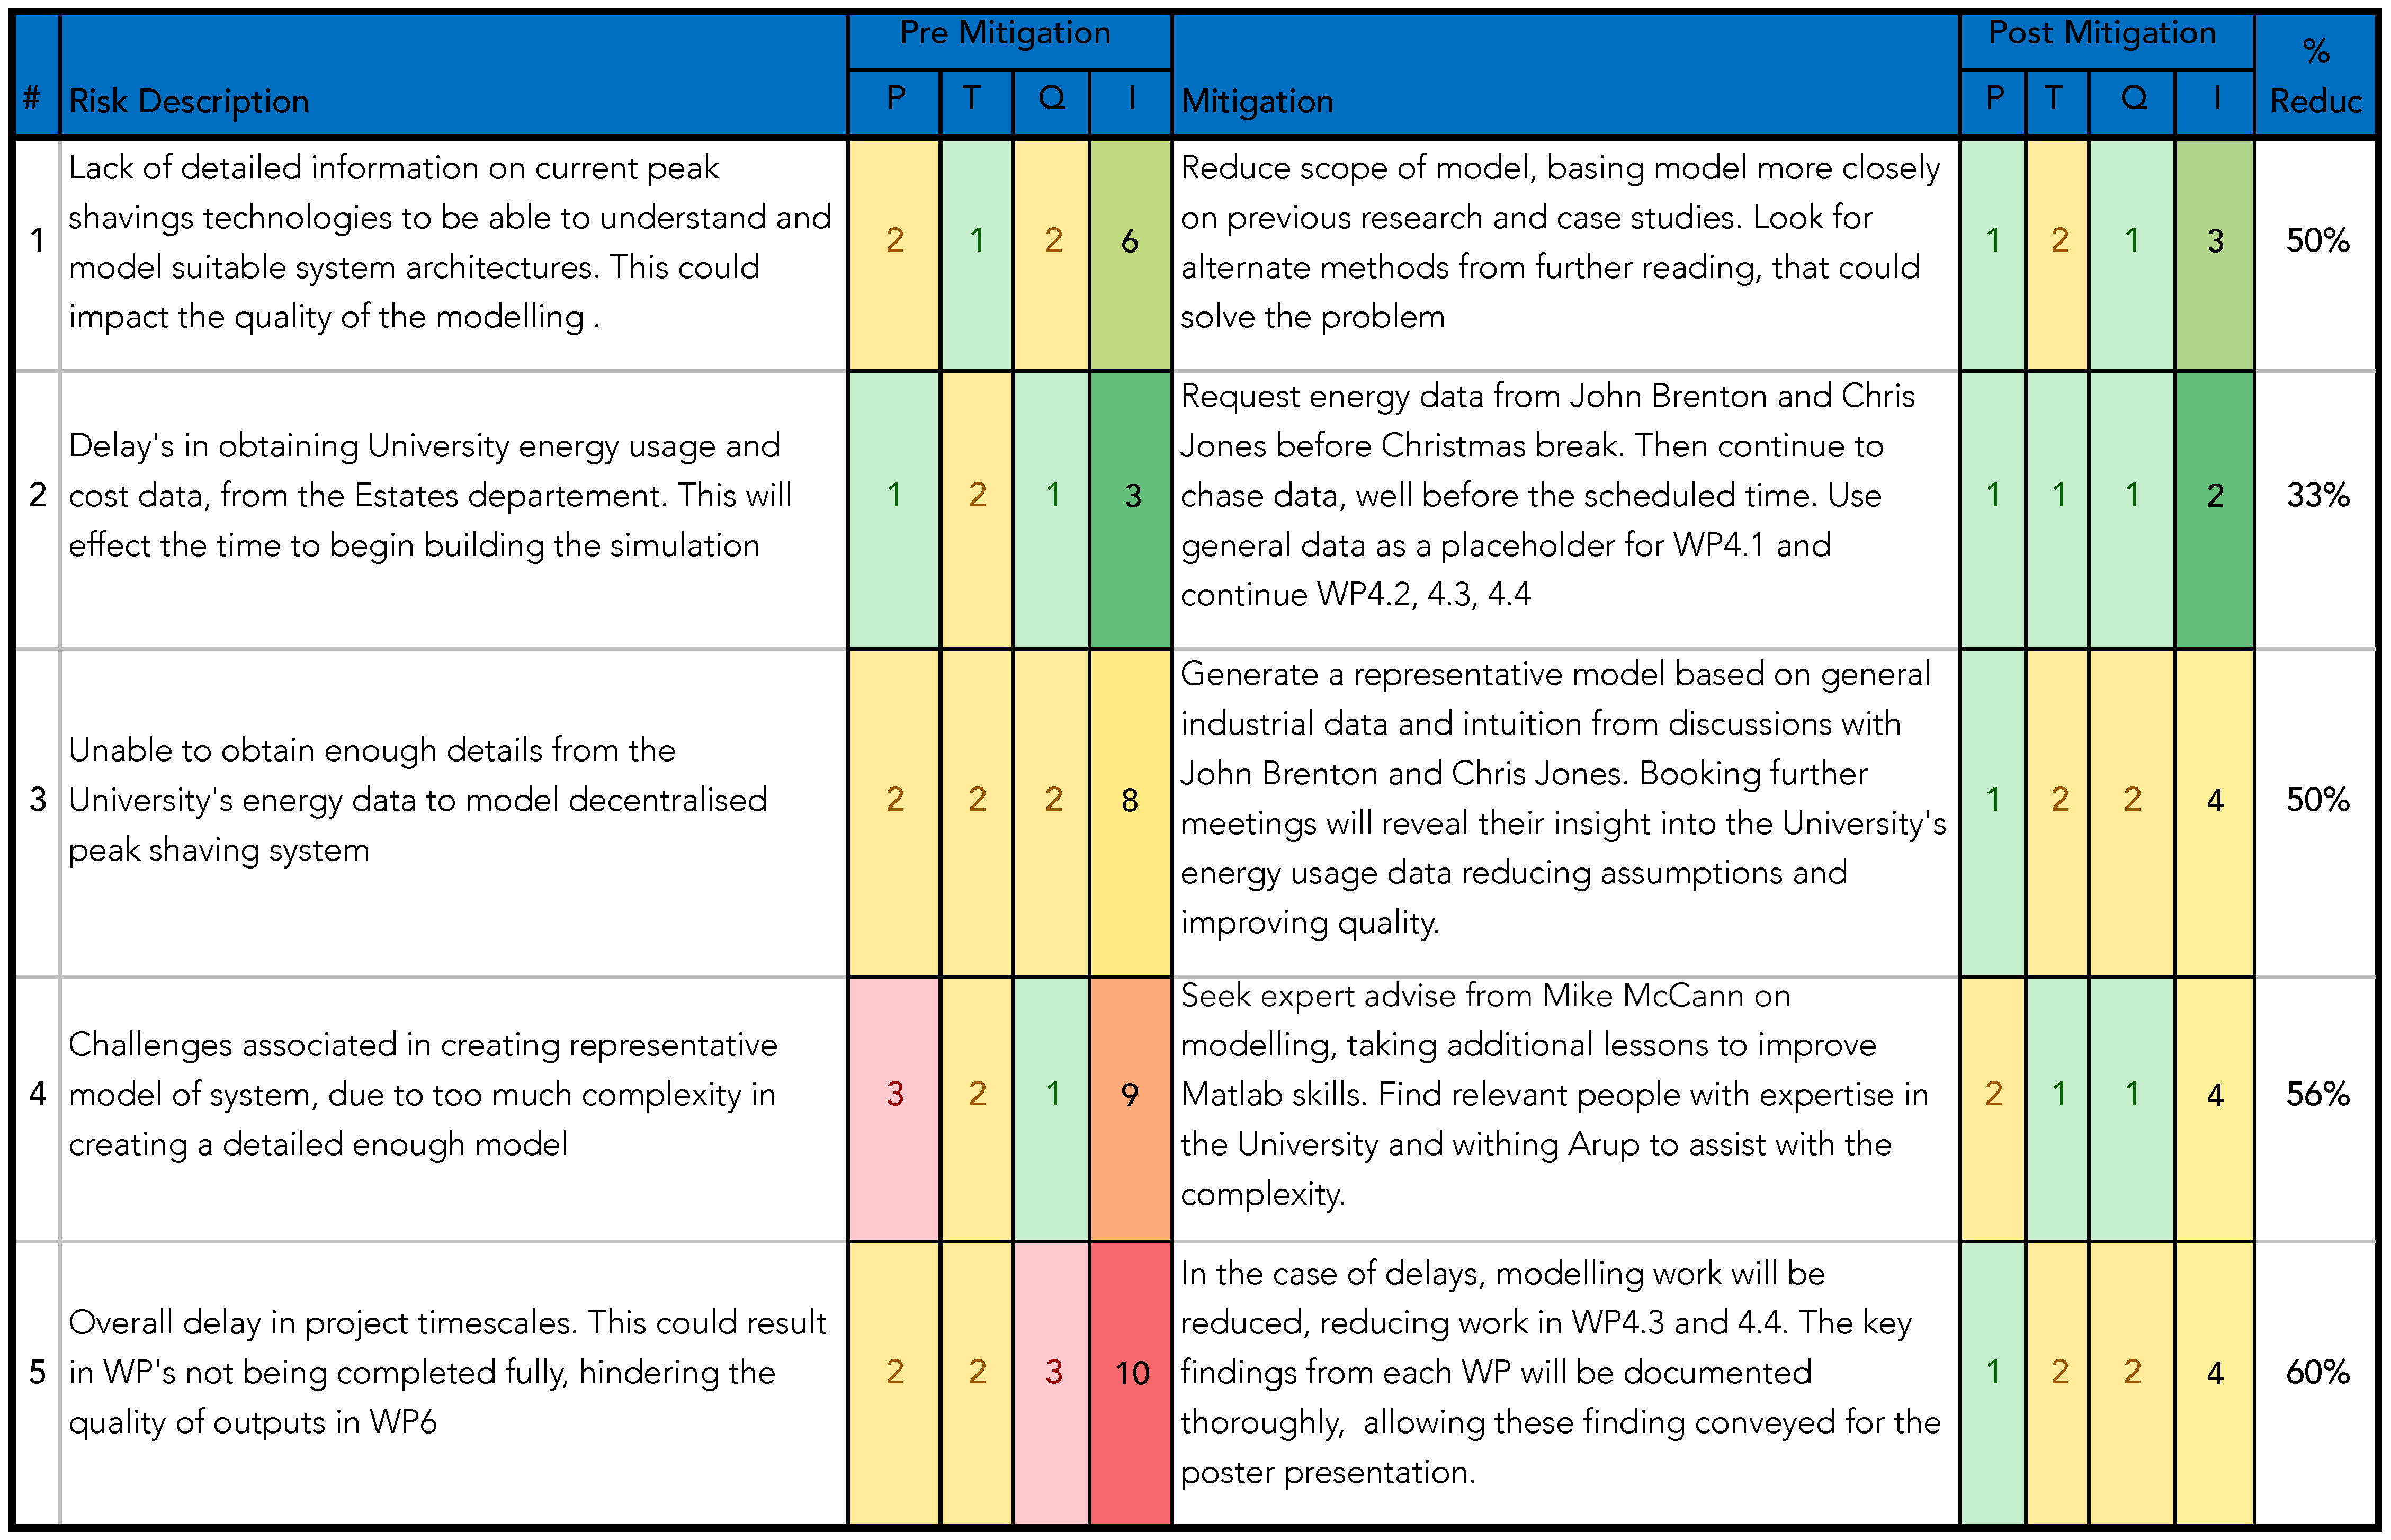
\includegraphics[height=0.8\textwidth]{risktab.eps}
\label{risktab}
\end{table}

\end{landscape}
% -----------------------------------------------------------------------------------
%                                  APENDIX
% -----------------------------------------------------------------------------------

\end{counted} %<<<<<<<<<<<<<<ENDS WORD COUNTER

\newpage
\section{Appendices}
Above were \thewords\ words. %<<<<<<<<<<<<<<DISPLAYS WORD COUNTER
% -----------------------------------------------------------------------------------
%                               BIBLIOGRAPHY - Insert Name of BIB File Here
% -----------------------------------------------------------------------------------
\newpage

% ---------------BIBTEX OLD-----------------------------------------------------
% \bibliographystyle{unsrt} %%%% Plain or alpha can change orders here
% \bibliography{BibFile}
 \nocite{*} %%%if you want to see all references even those note cited in the text
% -----------------------------------------------------------------------------------

\printbibliography

\end{document}
